\documentclass[aspectratio=169]{beamer}

% Custom theme and packages
\usepackage{beamertheme-custom}
% Custom symbols and commands
\usepackage{symbols-custom}

\graphicspath{{figures/}}

\title{Speeded response times}
\author{Joachim Vandekerckhove}
\date{Spring 2025}

% Font
\usefonttheme[onlymath]{serif}

\begin{document}

\maketitle

\begin{frame}[fragile]{Speeded response time}

Response times -- reaction times -- latencies\\[2ex]\pause

A very common type of data in experimental psychology
\pause

\bi
\i participants presented with a perceptual stimulus
\i asked to do a simple task like categorizing the stimulus (is this an `A' or a `B'?)
\i instructed to perform the task as quickly and accurately as possible
\i repeated many times with small variations or under different conditions
\ei

\end{frame}


\begin{frame}[fragile]{A few subtle distinctions: Speeded vs.\ not}
\vspace{-4ex}
\ex{Speeded response times}
These result from easy tasks where the participant is instructed to respond as quickly as possible.  They happen on short time scales -- \emph{less than a second on average}.  You might call them `split-second' decisions.  Real life examples are tasks such as deciding when to apply the brake while driving, or whether to duck or jump if an object flies your way.
\xe\pause

\vspace{-2ex}
\ex{Non-speeded response times}
These result from more complex tasks where the participant has to weigh many considerations and may have to deal with the consequences of a decision.  They happen on much slower time scales -- \emph{at least several seconds} but possibly much longer.  They include decisions such as economic decisions (e.g., buying a car) or social decisions (e.g., how to respond to a marriage proposal).
\xe

\end{frame}



\begin{frame}[fragile]{A few subtle distinctions: Simple vs.\ choice}

\ex{Choice response times}
These result from tasks in which the participant is specifically instructed to choose between several alternatives.  They not only have to press a button but additionally have to \emph{choose which button} to press.  There may be two alternatives (two-choice response times) or more than two (multiple-choice or multialternative response times).  Note that choice response times are \emph{bivariate}.
\xe\pause

\ex{Simple response times}
These result from tasks where there is no ambiguity about which button to press -- the instruction is simply to press it as quickly as possible.  Simple response times are \emph{univariate}.
\xe

\end{frame}


\begin{frame}[fragile]{The strangeness of choice response times}

\begin{figure}[htp]
\centering
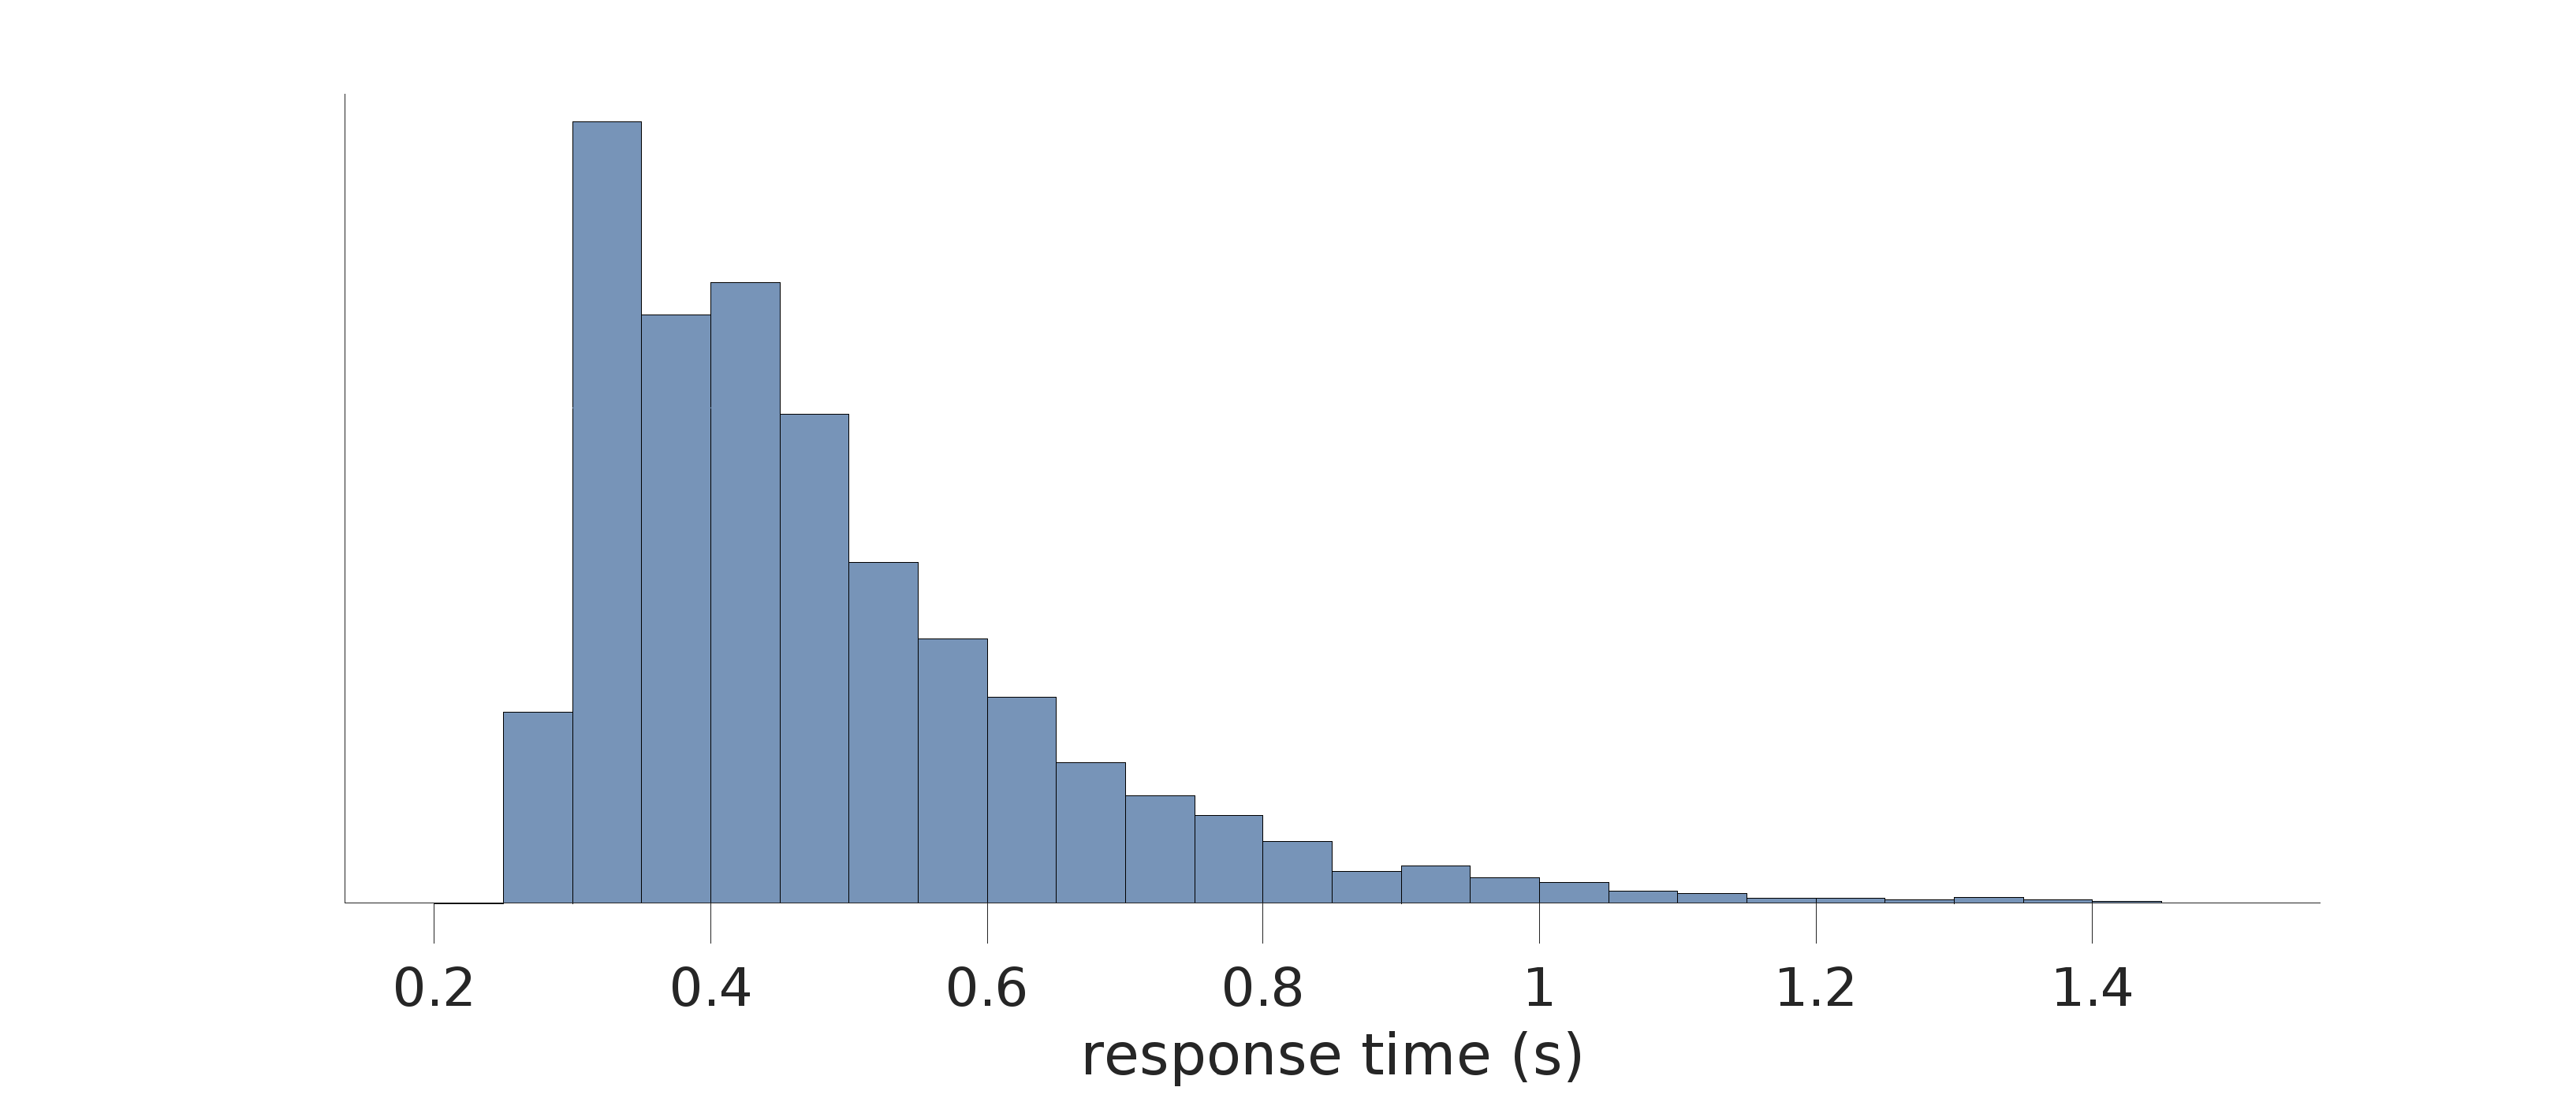
\includegraphics[scale=0.2]{rtdist}
\end{figure}

\bi
\i Non-normal and skewed
\i `Hard left bound'
\ei

\end{frame}


\begin{frame}[fragile]{The strangeness of choice response times}

\begin{figure}[htp]
\centering
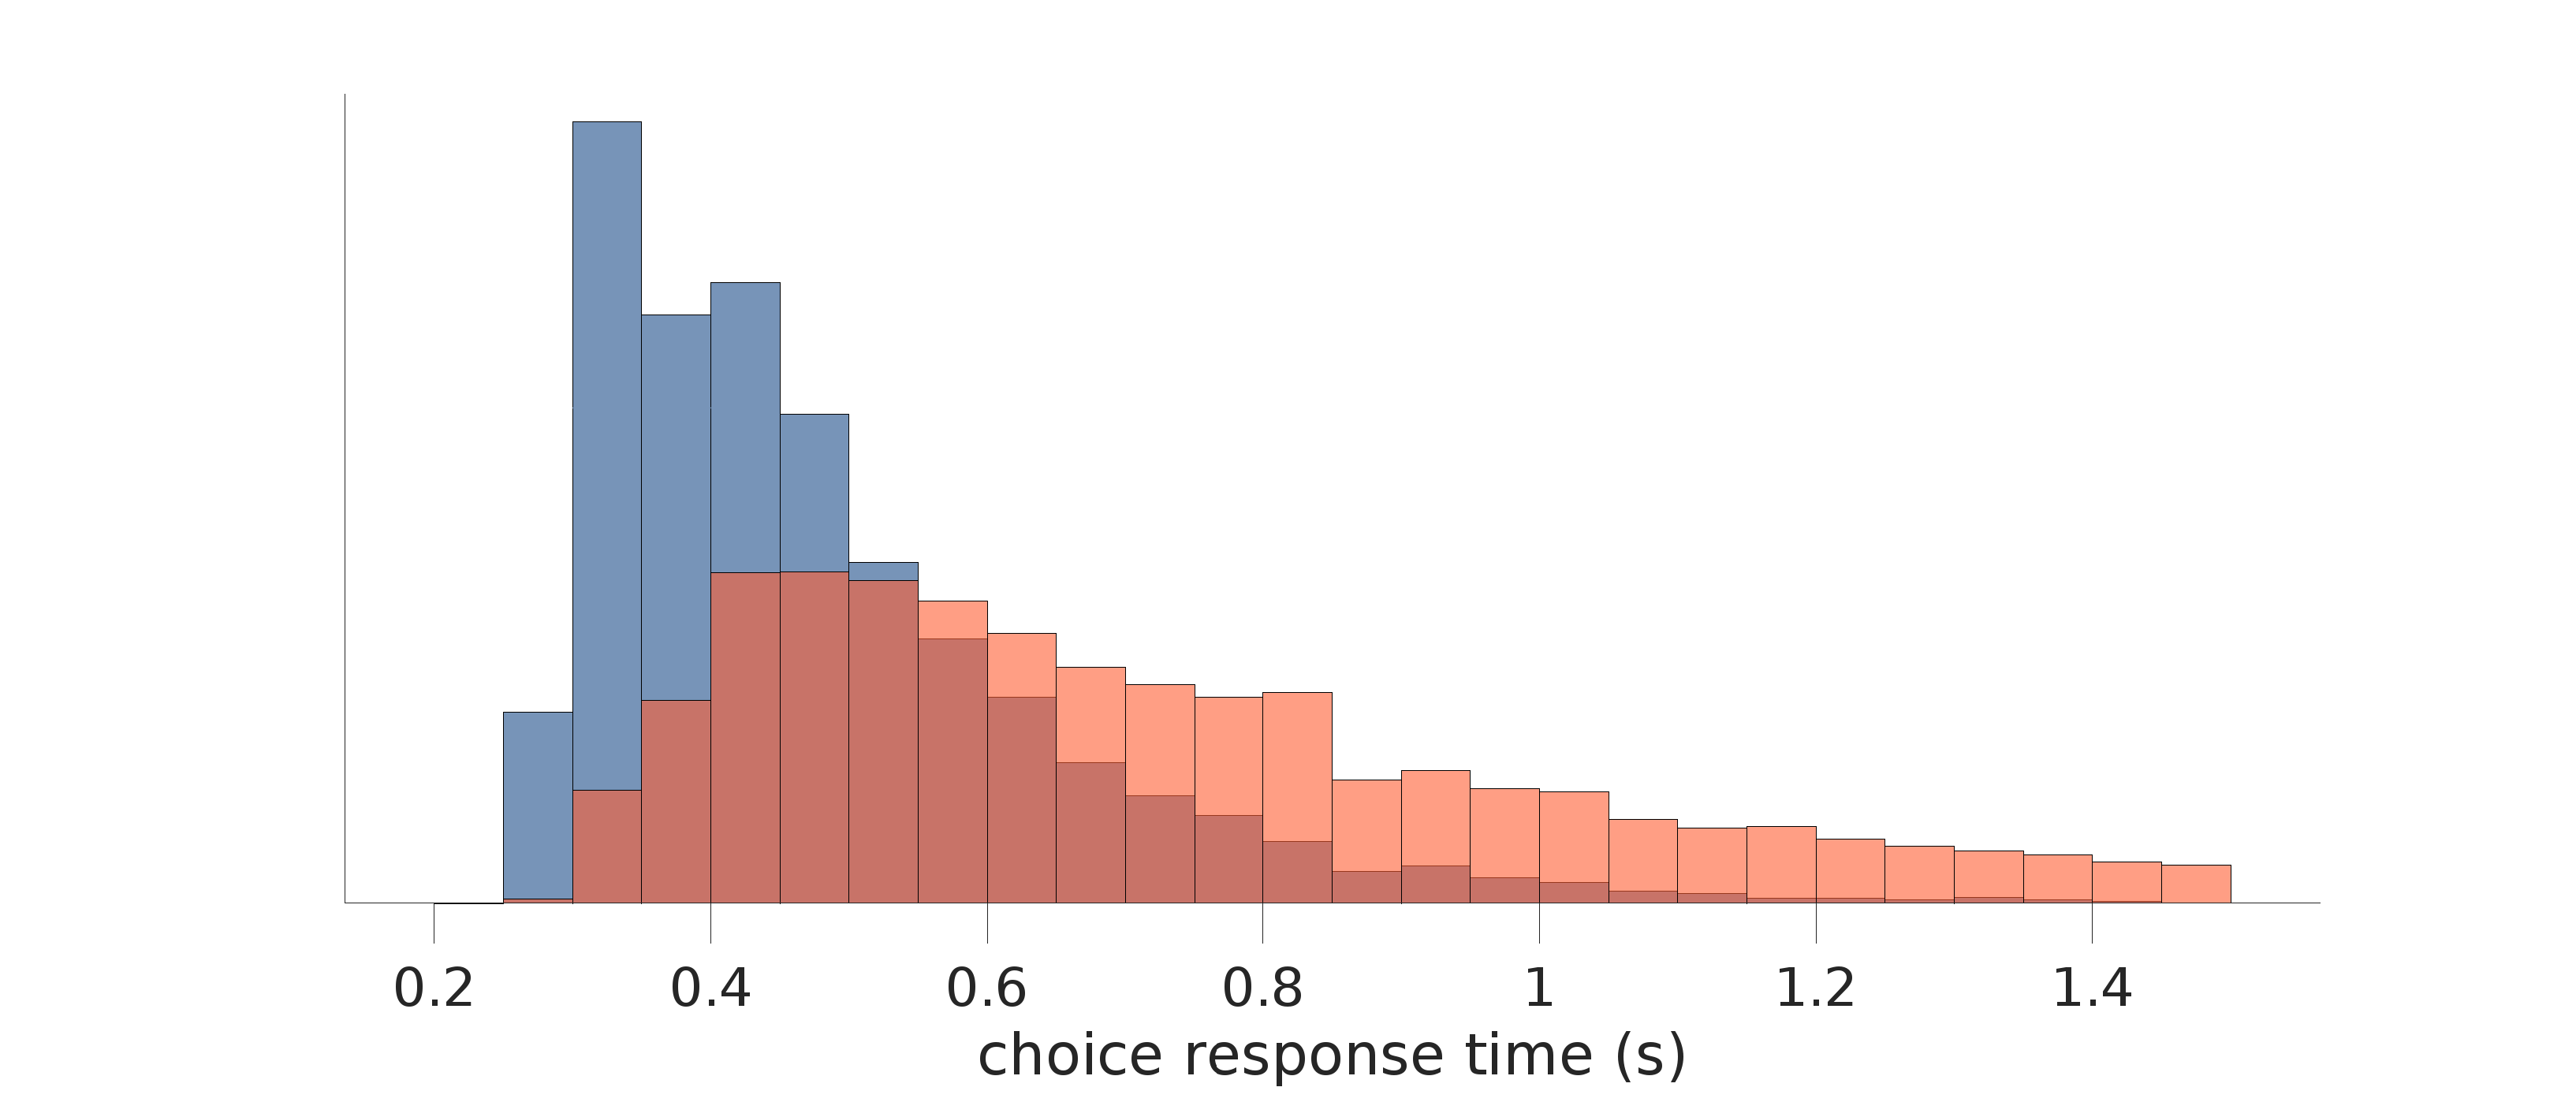
\includegraphics[scale=0.2]{rtdist2}
\end{figure}

\bi
\i Bivariate (one continuous, one binary)
\i Not independent
\ei

\end{frame}


\begin{frame}[fragile]{Summaries of CRTs}

\begin{figure}[htp]
\centering
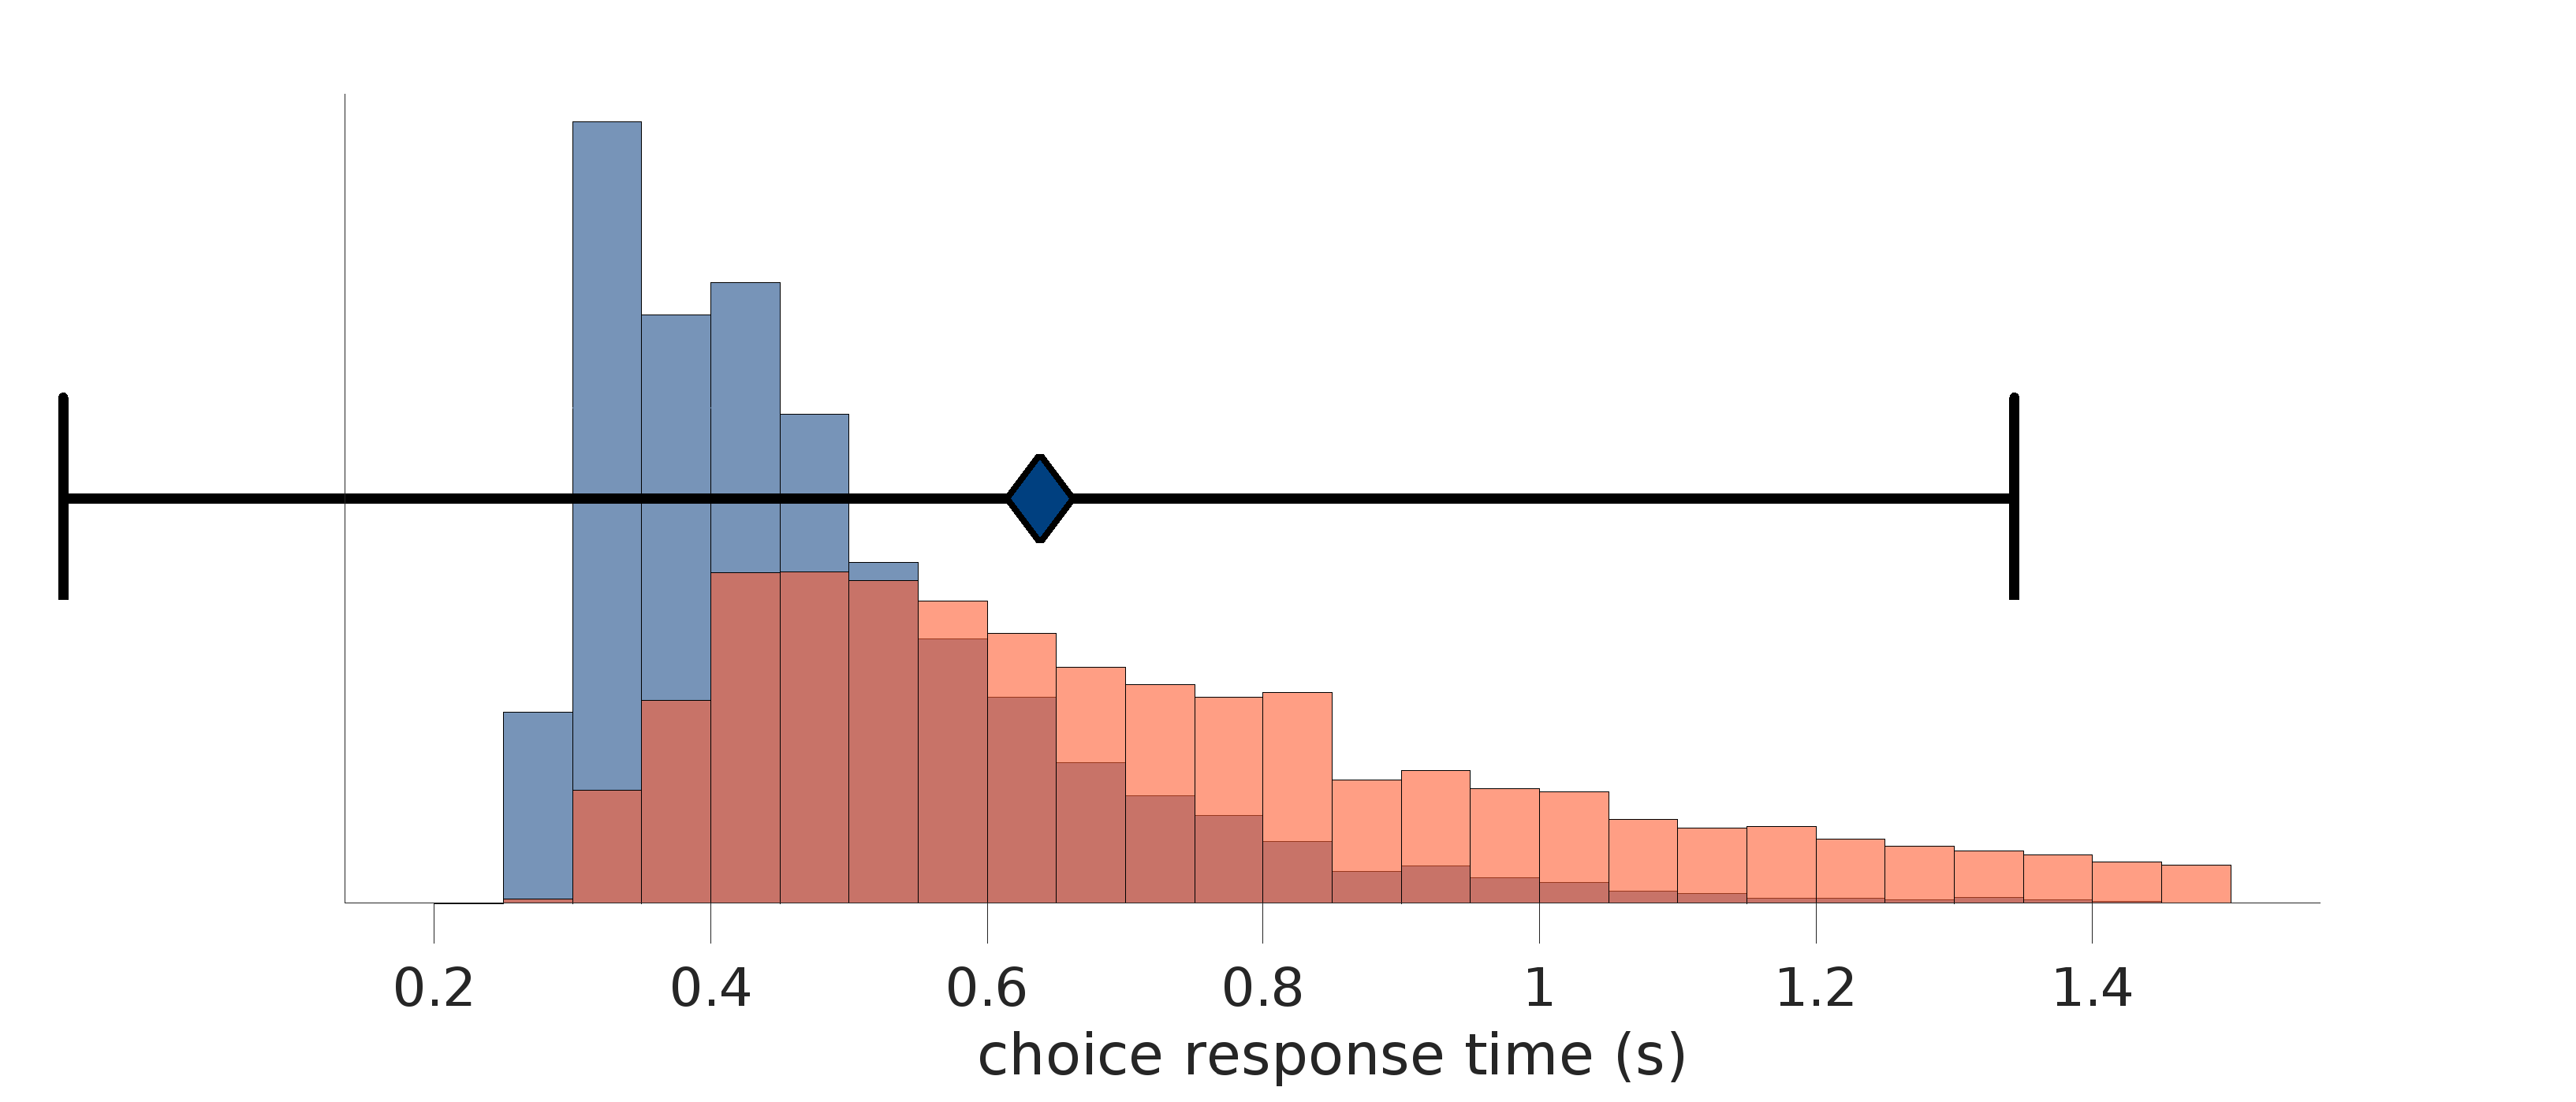
\includegraphics[scale=0.2]{rtdist3}
\end{figure}

\bi
\i Are mean and SD really capturing the information in these data?
\i Here the 95\% CI goes into the negative
\ei

\end{frame}



\begin{frame}[fragile]{Variance stabilization}

It is possible to give a strictly statistical treatment to the skewed data through various \emph{variance stabilizing transformations}.\\[2ex]

\begin{figure}[htp]
\centering
\includegraphics<1>[scale=0.2]{rtdist4}%
\includegraphics<2>[scale=0.2]{rtdist5}
\end{figure}

\end{frame}



\begin{frame}[fragile]{Visualizing CRT data}

CRT distributions can have a lot of detail and information in them

\begin{figure}[htp]
\centering
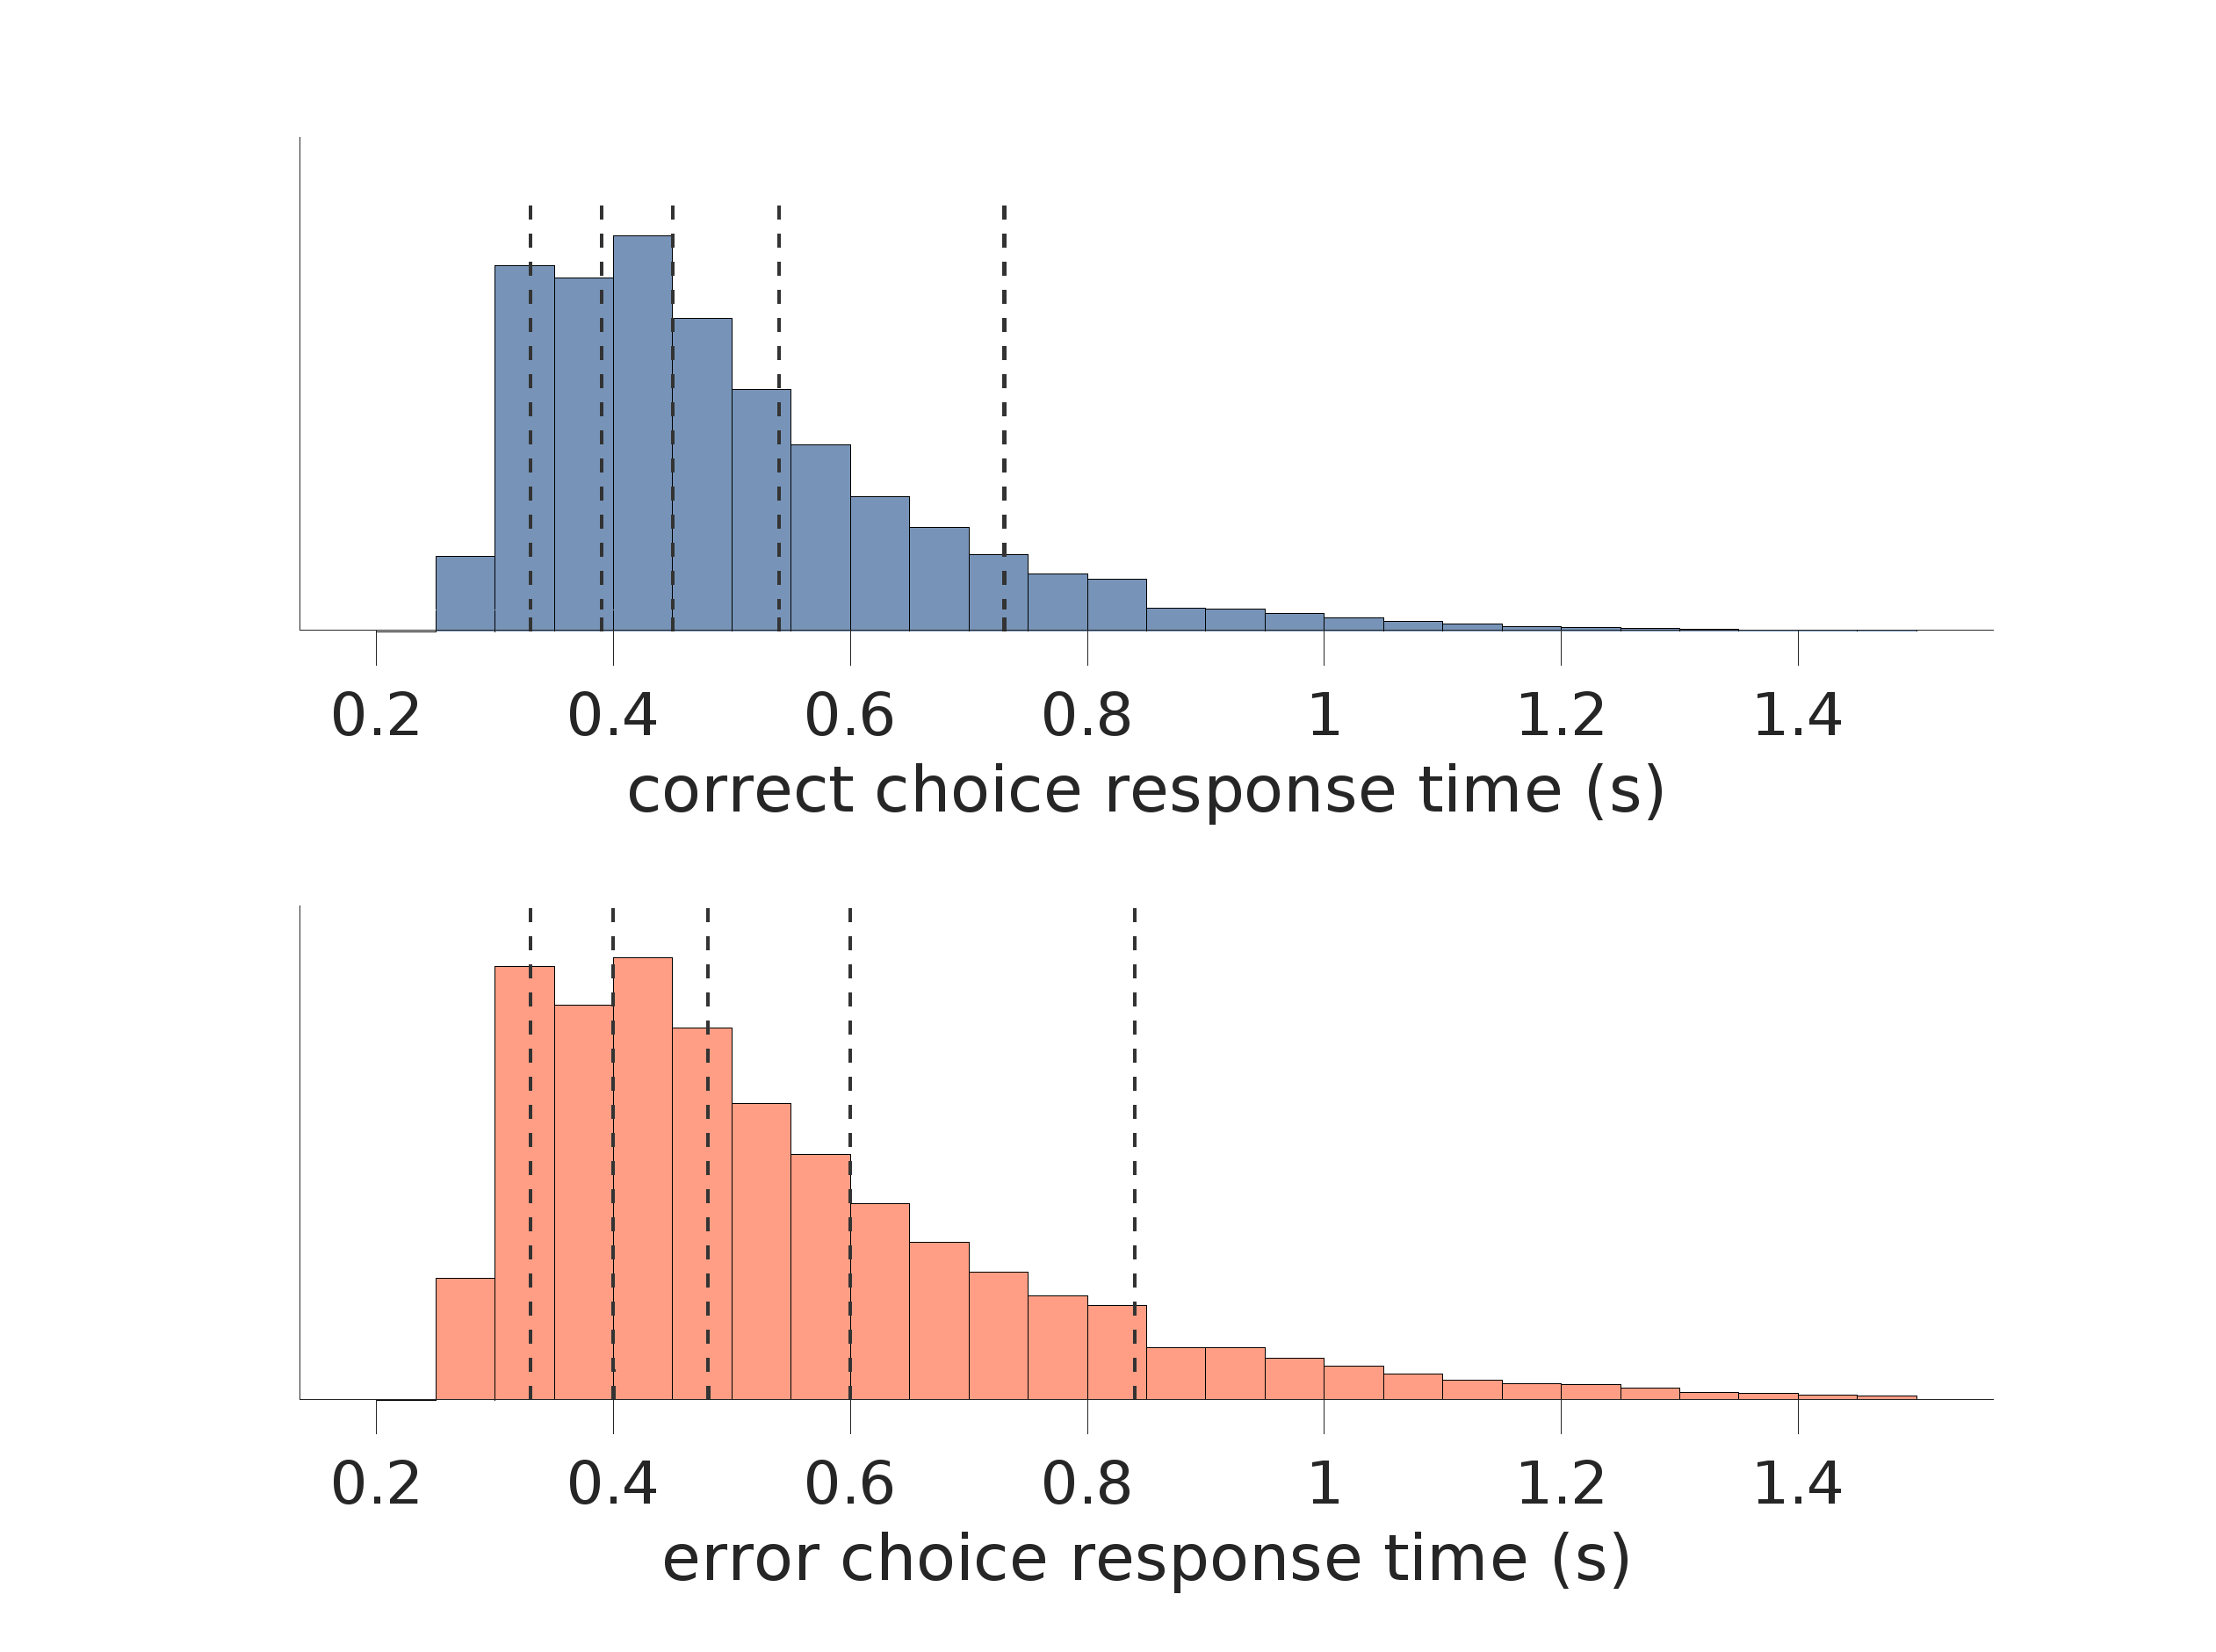
\includegraphics[scale=0.2]{rtdist6}
\end{figure}

\end{frame}



\begin{frame}[fragile]{Visualizing CRT data}

\bi
\i What is the proportion of errors?
\i Do errors have higher variance?
\i Does an experimental manipulation affect errors and correct responses similarly?
\i Does an experimental manipulation all quantiles similarly?
\ei

\end{frame}


\begin{frame}[fragile]{Visualizing CRT data}
\vspace{-3ex}
\emph{Quantiles} can be used to summarize nonstandard distributions\pause

Here, each distribution is marked with the
$10^\text{th}$,
$30^\text{th}$,
$50^\text{th}$,
$70^\text{th}$, and
$90^\text{th}$, percentile, so that 20\% of the data falls in each of the middle bins\pause
\begin{figure}[htp]
\centering\vspace{-4ex}
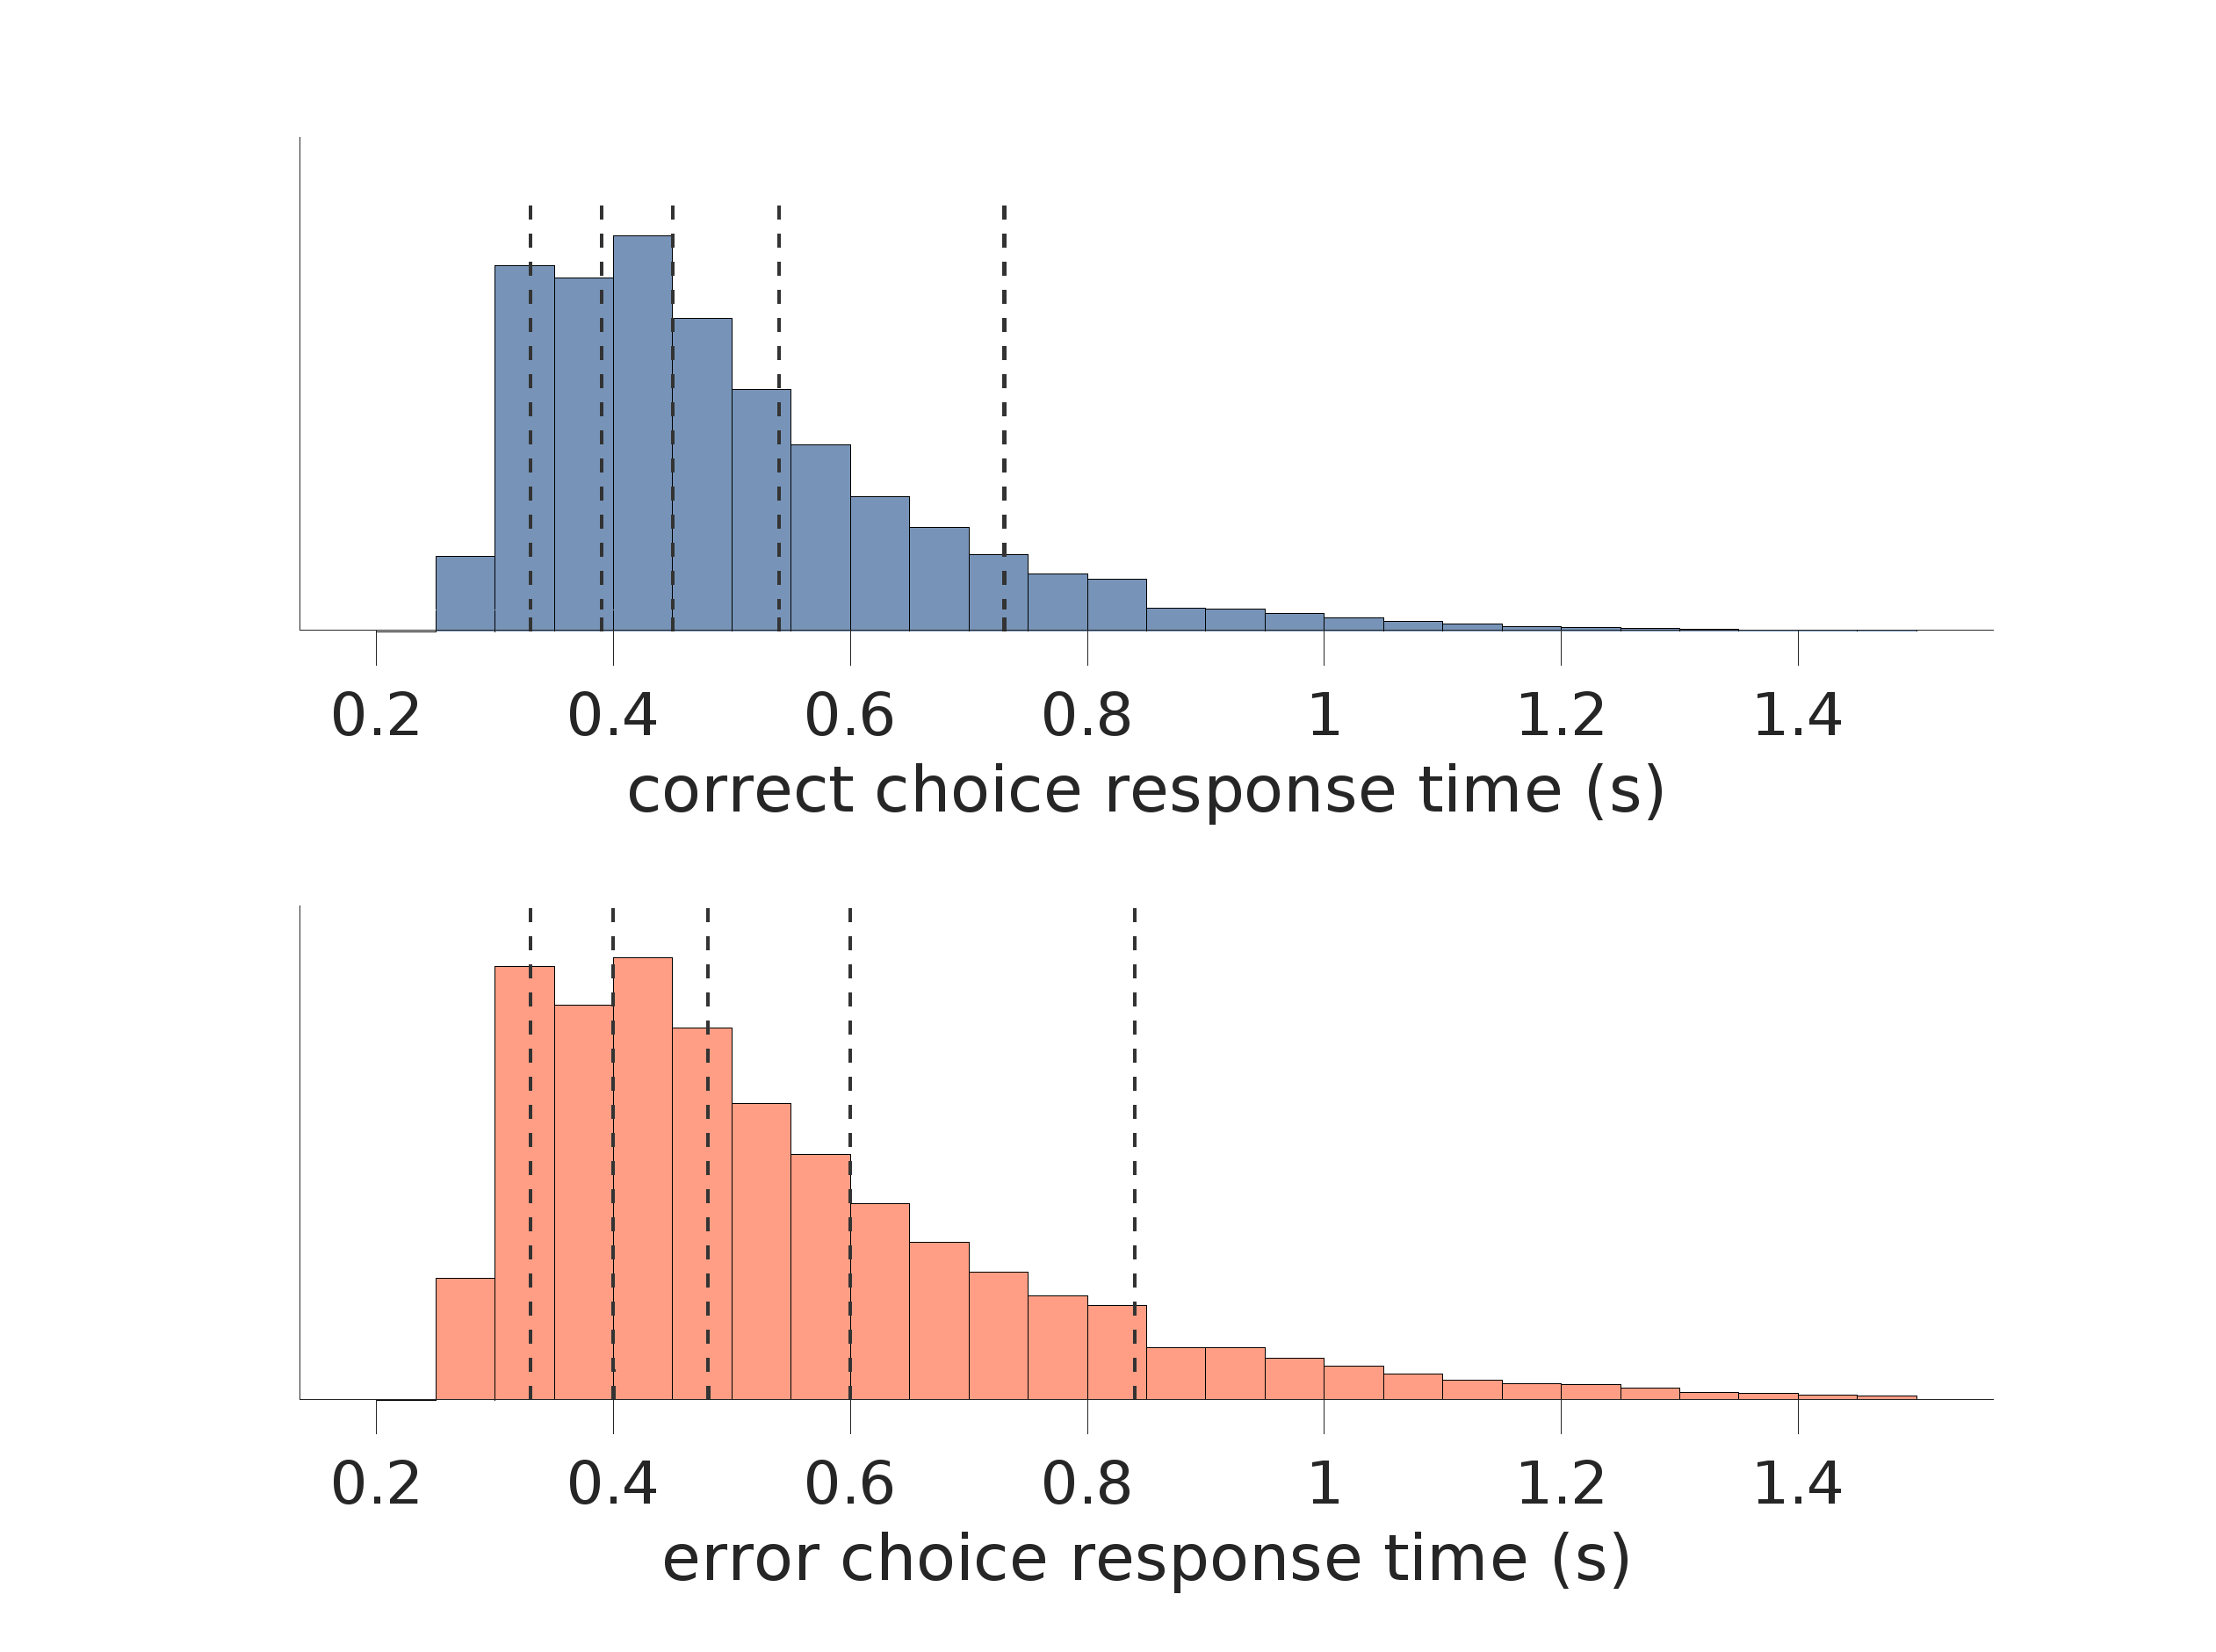
\includegraphics[scale=0.2]{rtdist6}
\end{figure}

\end{frame}

\begin{frame}[fragile]{Quantile probability plots \cite{Simen2009}}

Plot the RT quantiles (vertical) over the condition accuracy (horizontal)

\begin{figure}[htp]
{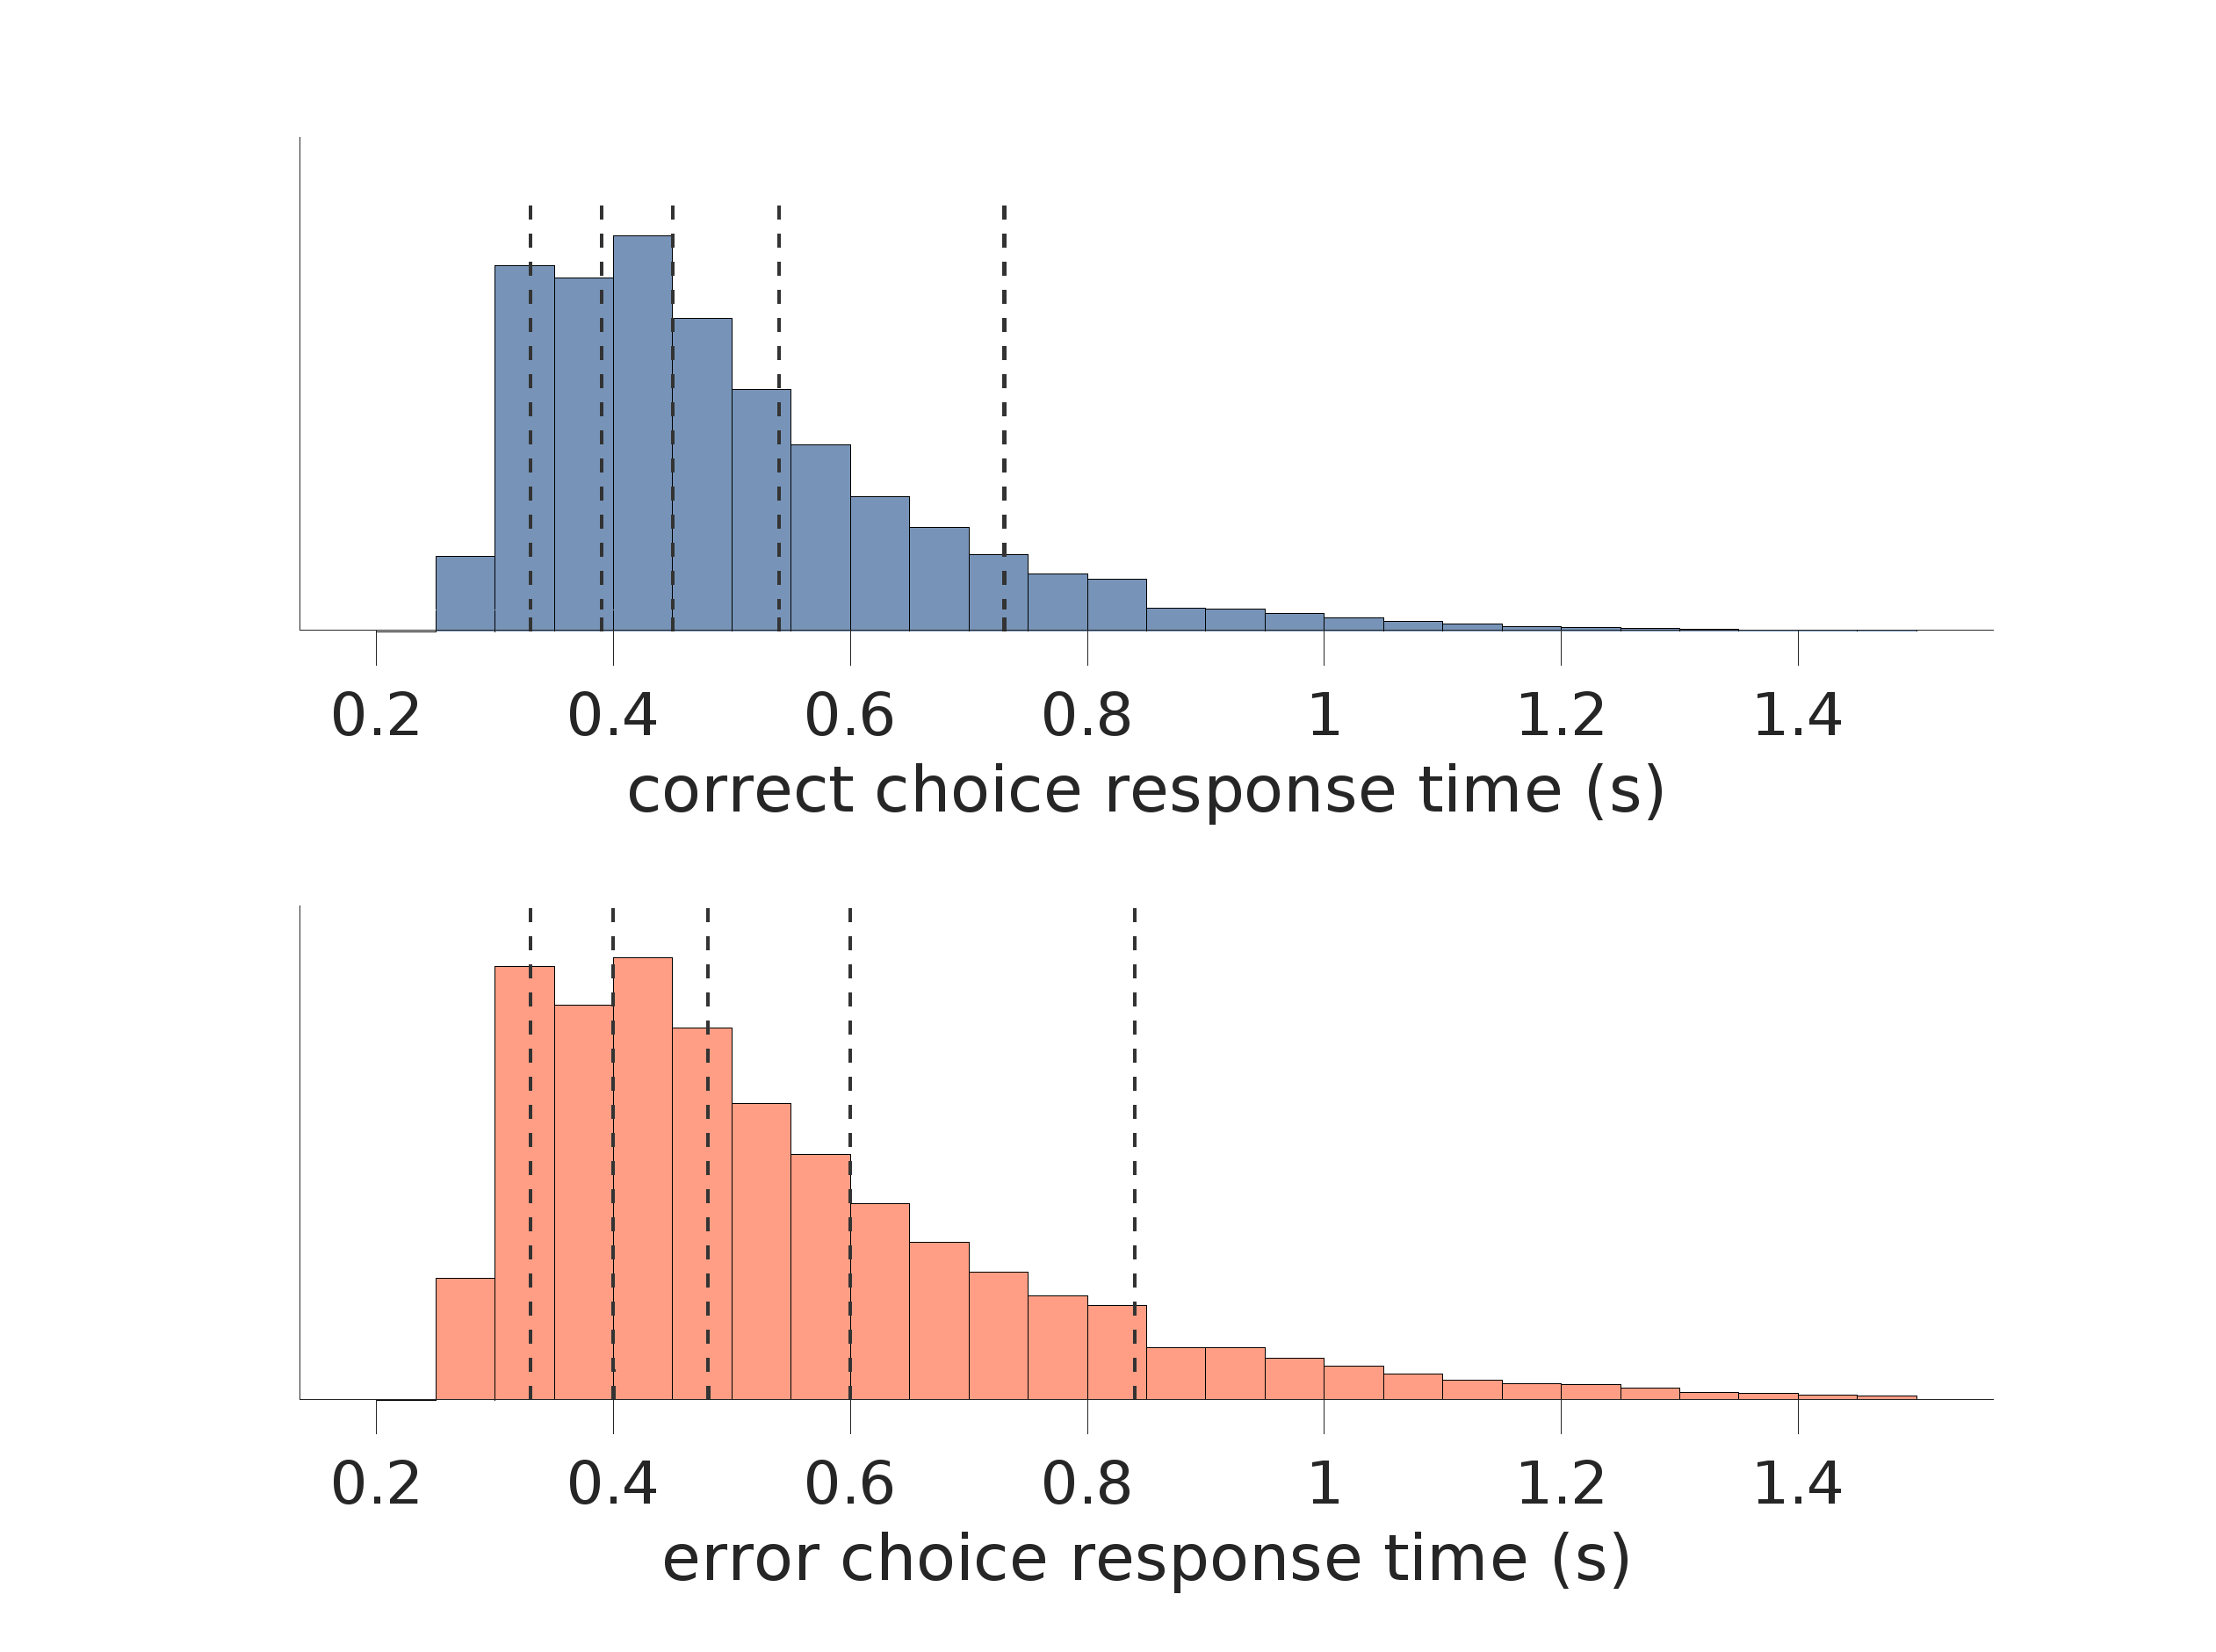
\includegraphics[scale=0.122, bb=110 -20 1400 640,angle=90,clip]{rtdist6}}
{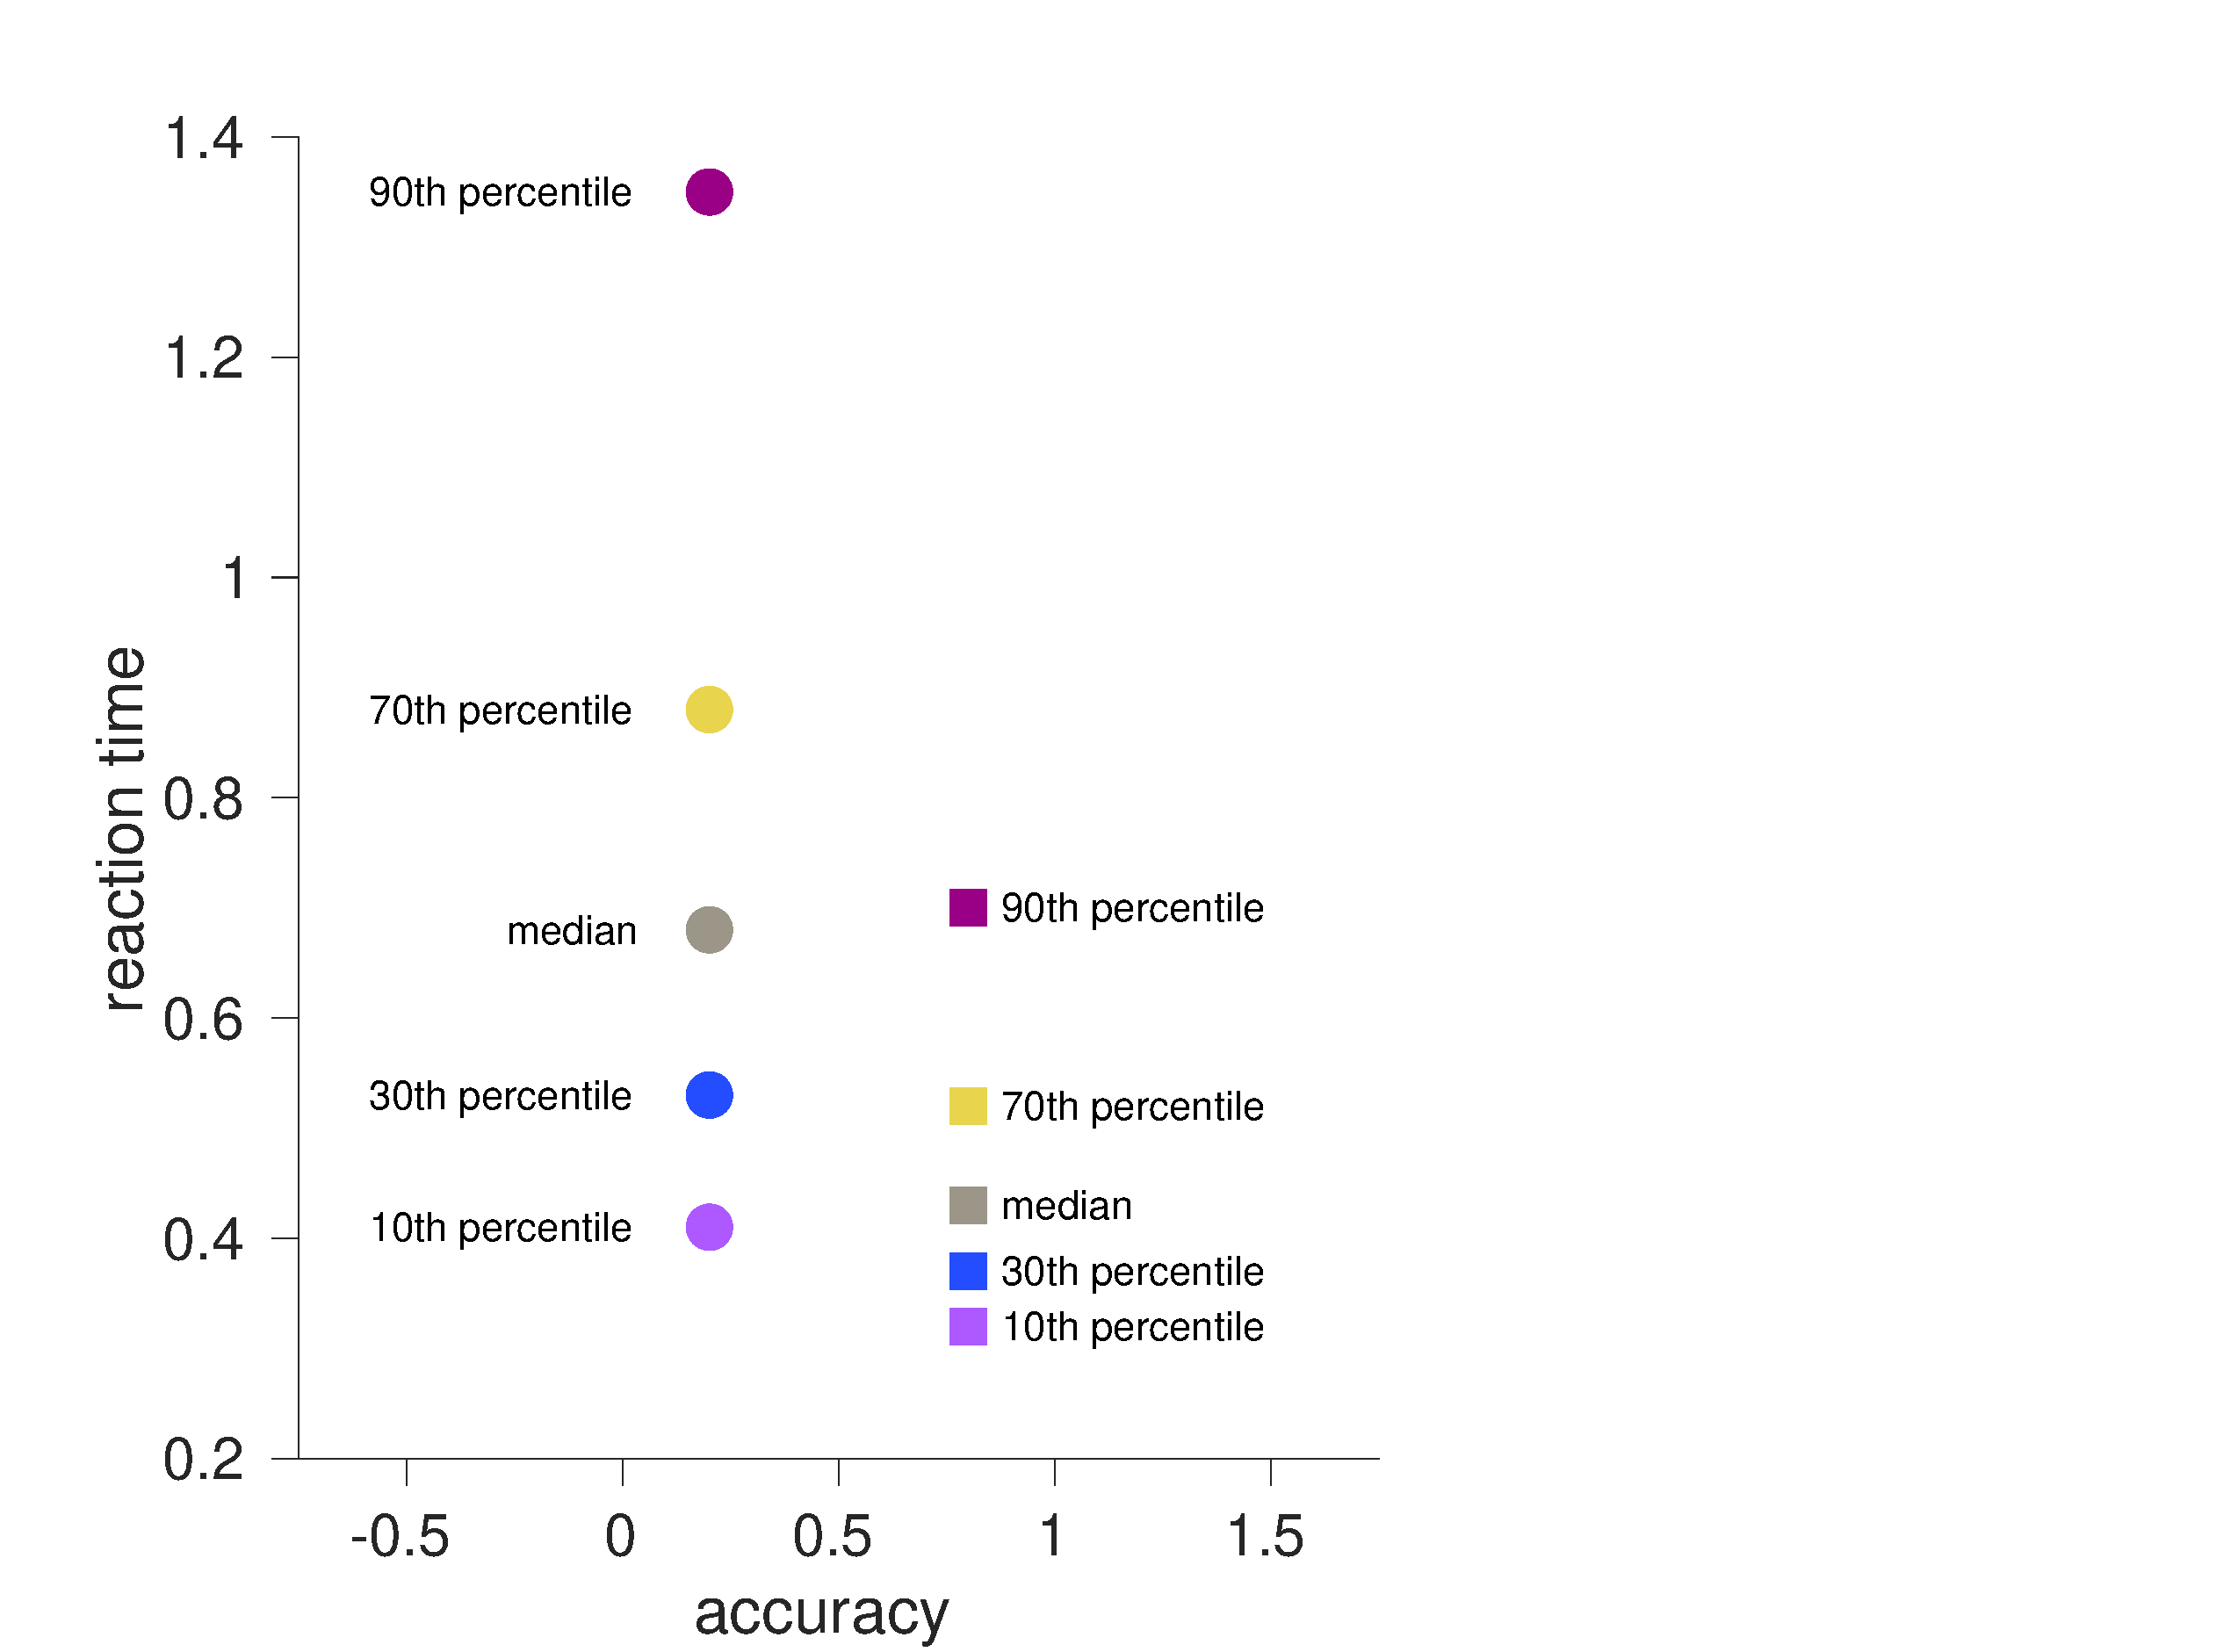
\includegraphics[scale=0.235, bb=60 0 925 640,clip]{rtdist7}}
\end{figure}

\end{frame}



\begin{frame}[fragile]{Quantile probability plots \cite{Simen2009}}

\begin{flushright}\footnotesize
(Data from \citeNP{vandekerckhove_etal:2007:concavity})
\end{flushright}
\begin{figure}[htp]
\centering
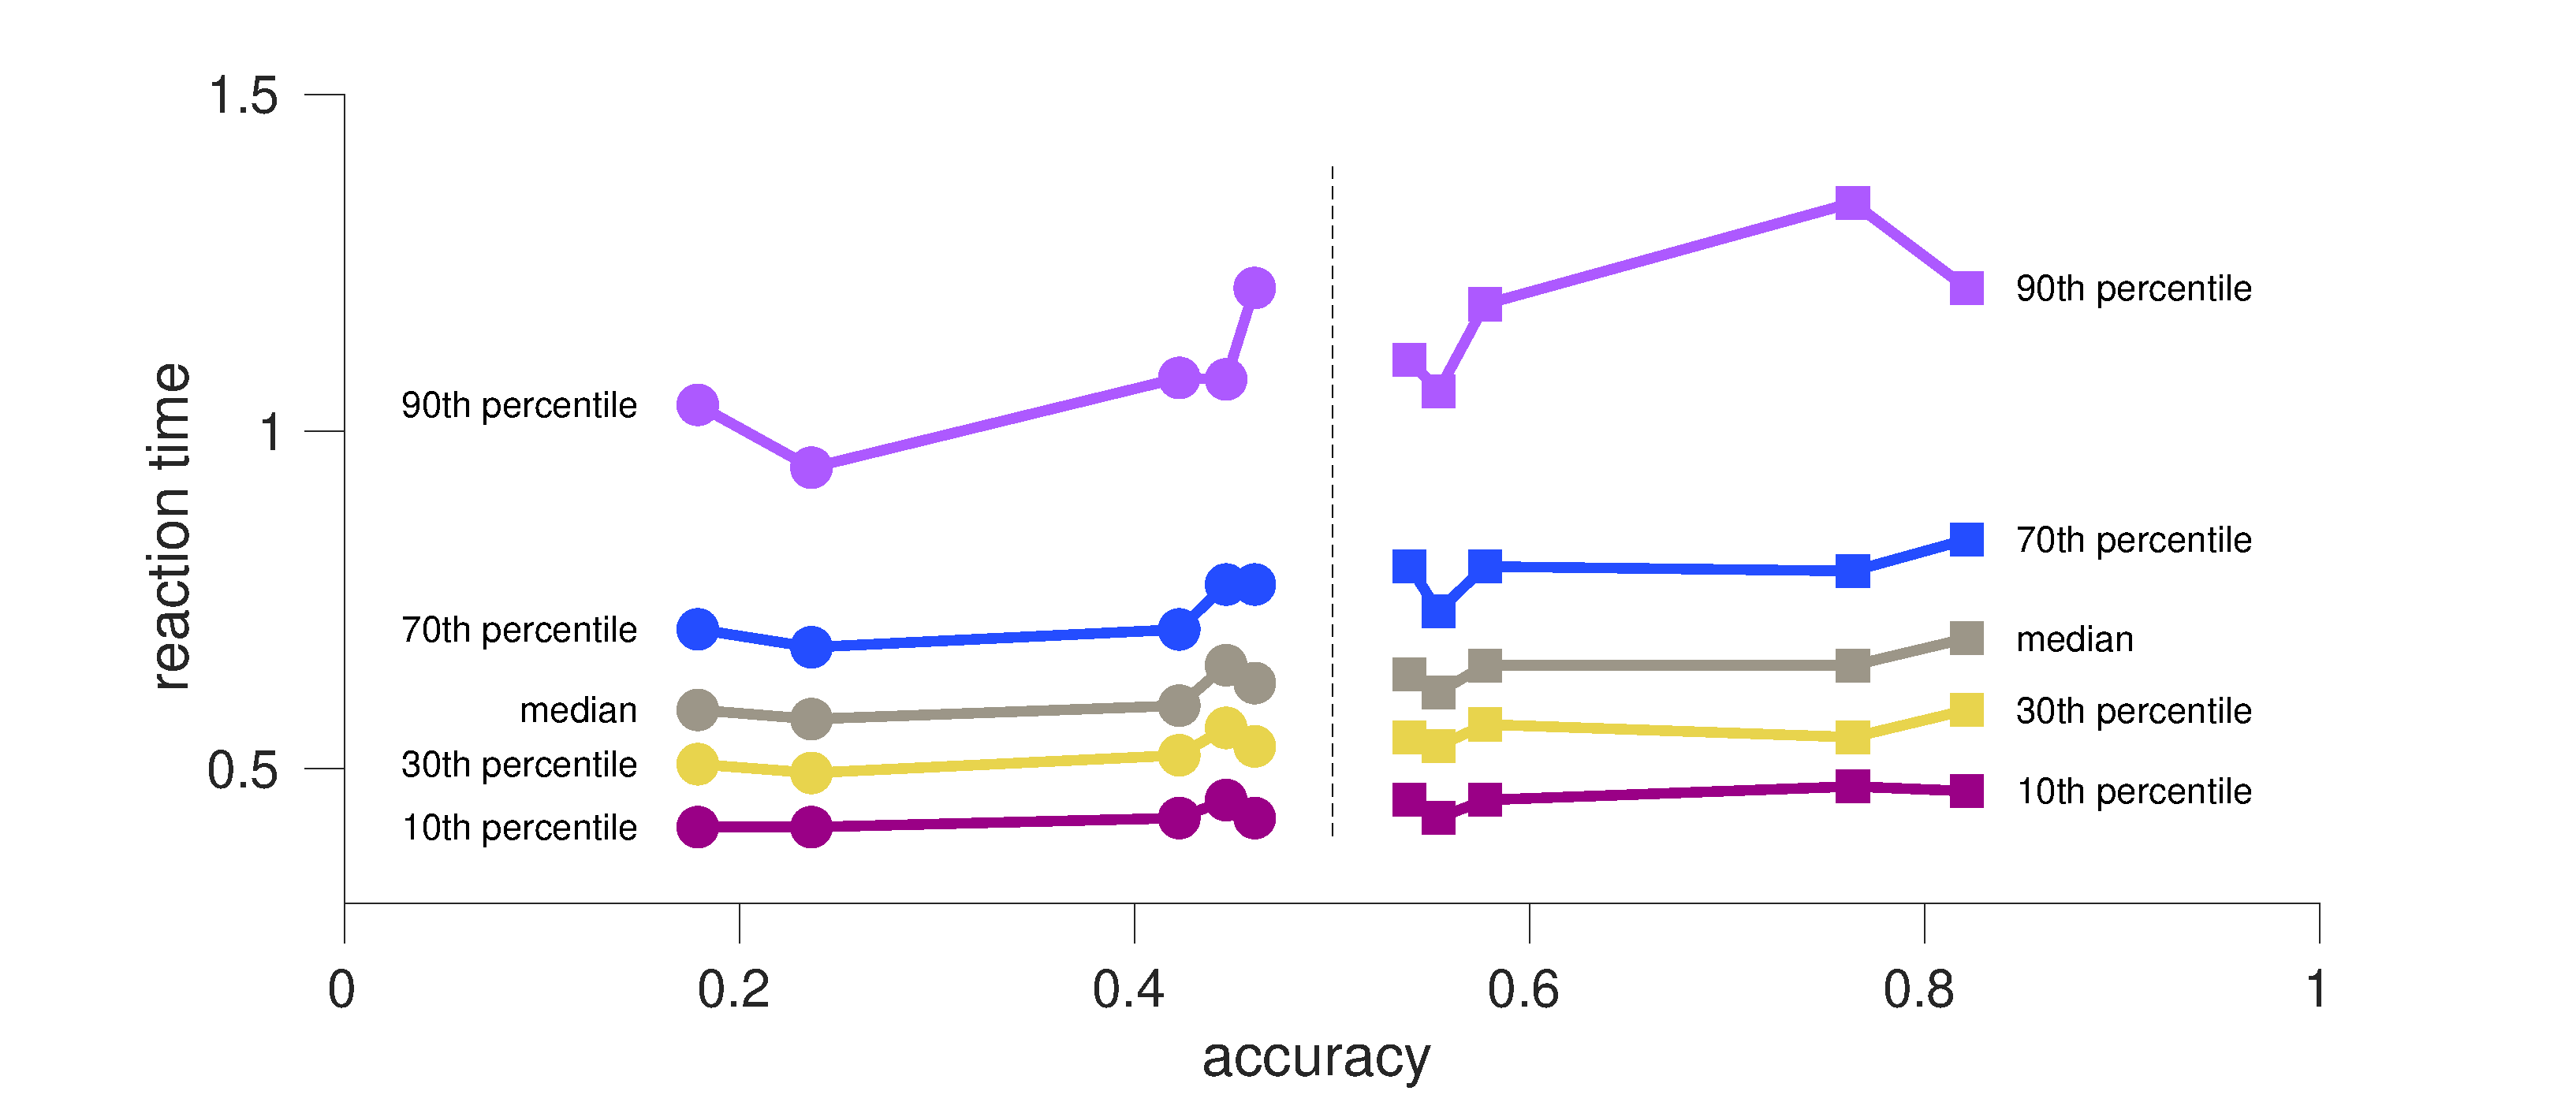
\includegraphics[width=\textwidth]{qppsp.eps}
\end{figure}\pause

\bi
\i show more detailed distributional information
\bi
\i does the manipulation affect fast and slow RTs the same?
\ei
\i show the bivariate nature of the data
\bi
\i does the manipulation affect correct and error RTs the same?
\ei
\ei
\end{frame}



\begin{frame}[fragile]{Direct comparison of quantiles}
\only<1->{QPP can be used to compare many conditions at once}

\only<2->{But they still rely on `visual arithmetic'}

\only<3->{\emph{Delta plots} visualize the difference in distribution between two conditions}
\begin{figure}[htp]
\centering
\includegraphics<4>[width=.8\textwidth]{deltasmall0.eps}%
\includegraphics<5>[width=.8\textwidth]{deltasmall1.eps}%
\includegraphics<6>[width=.8\textwidth]{deltasmall2.eps}
\end{figure}
\only<6>{$$\Delta_n = P_n(t_2) - P_n(t_1)$$}

\end{frame}



\begin{frame}[fragile]{Delta plots \cite{Pratte2010}}
\begin{minipage}{.35\textwidth}\centering
\begin{tabular}{cc}
$\Delta_{10} = 0.05$\\
$\Delta_{30} = 0.08$\\
$\Delta_{50} = 0.11$\\
$\Delta_{70} = 0.13$\\
$\Delta_{90} = 0.17$\\
\end{tabular}
\end{minipage}
\begin{minipage}{.55\textwidth}
\begin{figure}[htp]
\centering
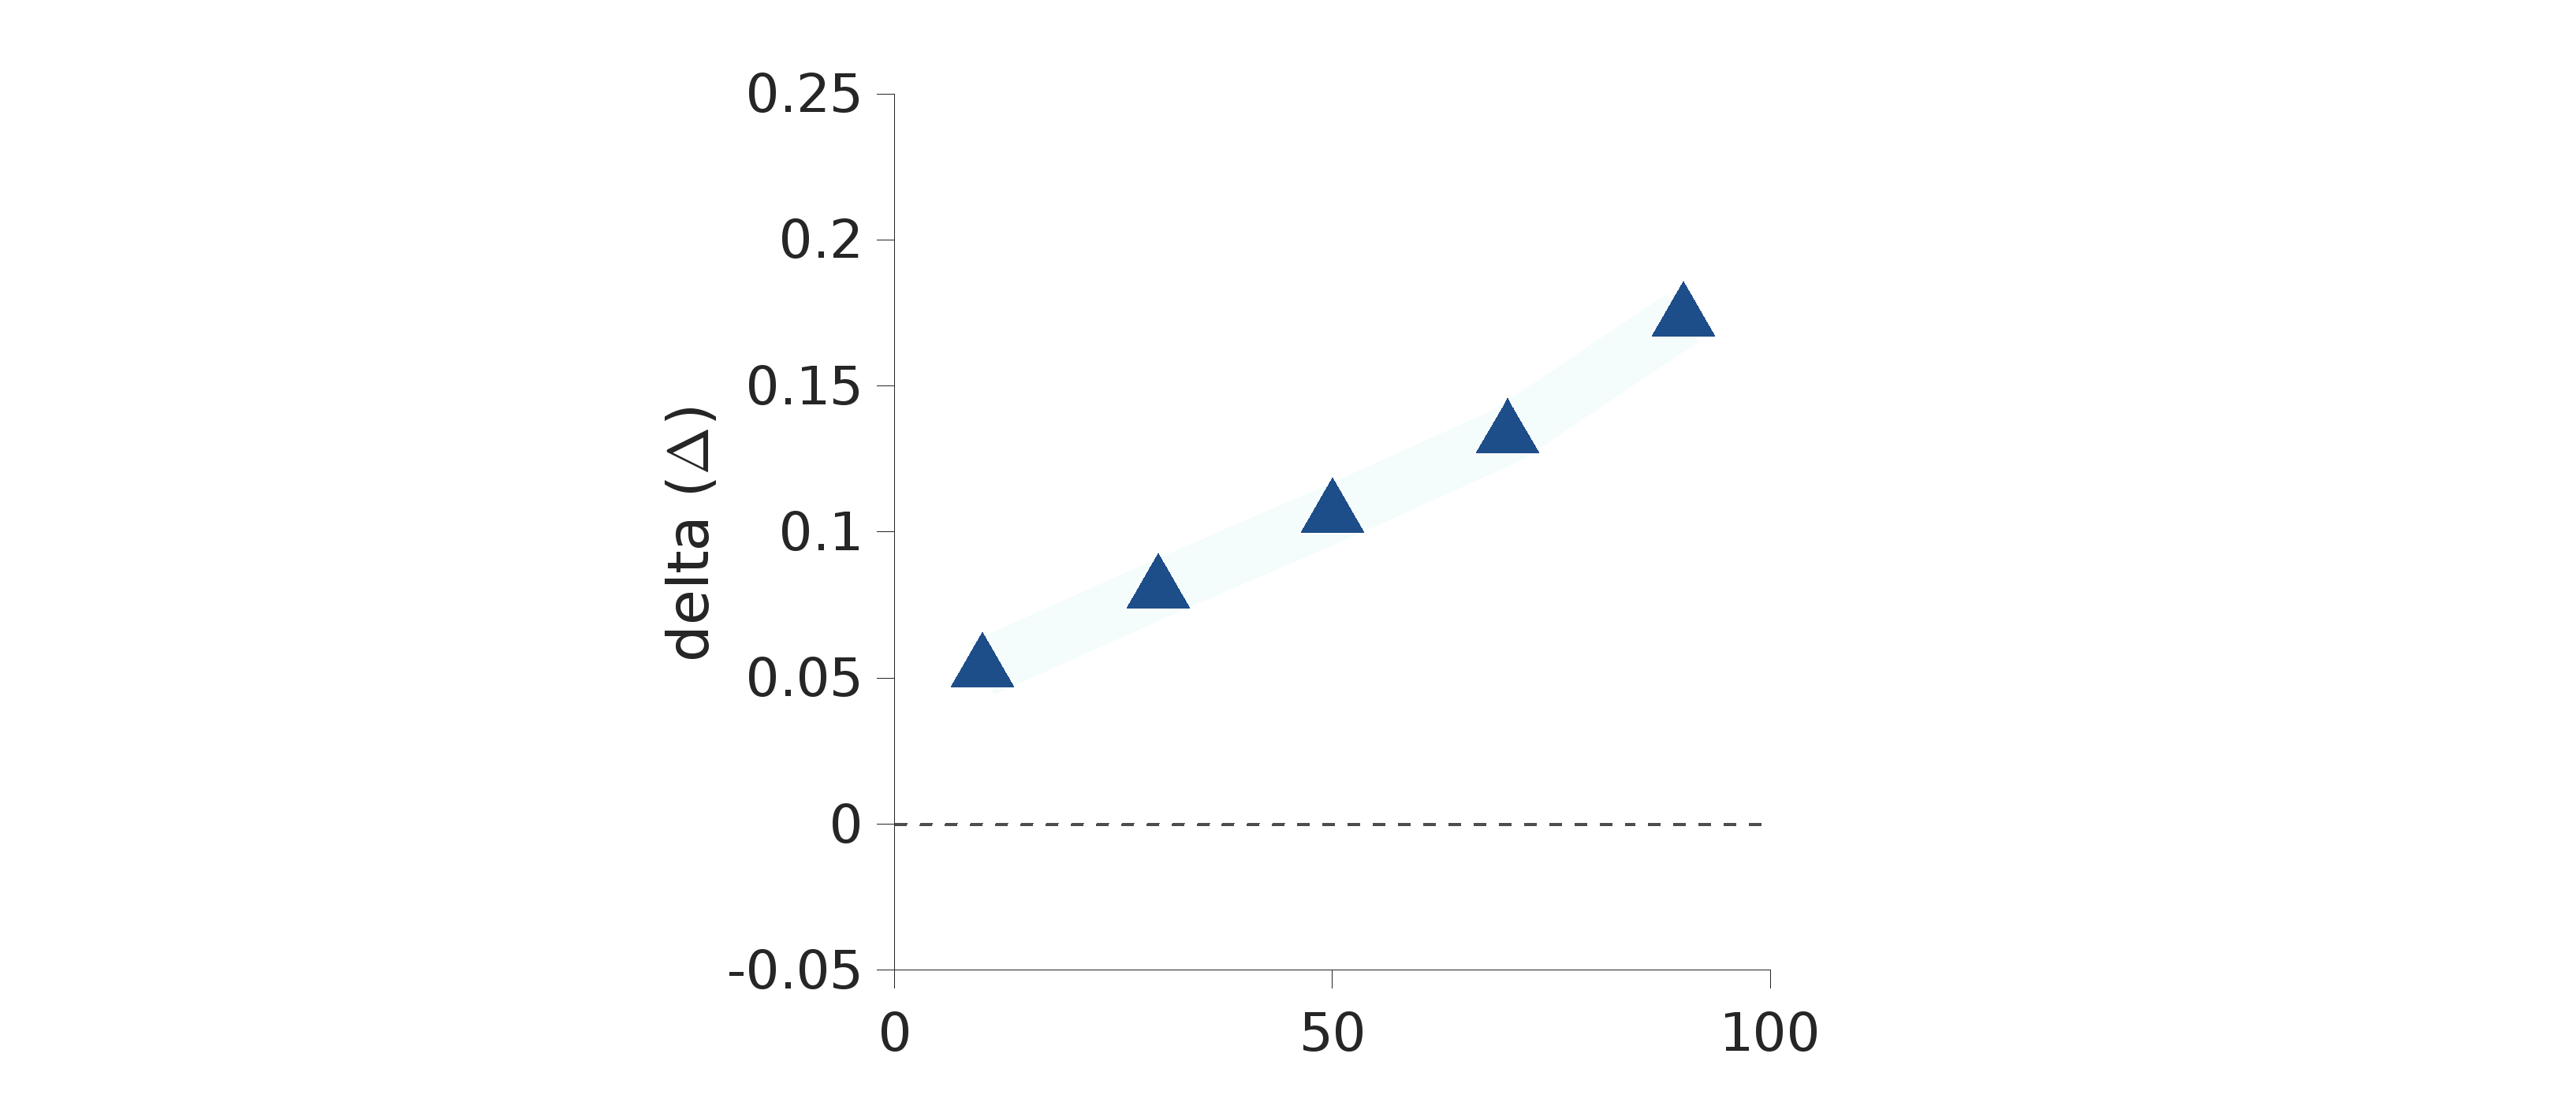
\includegraphics[scale=0.2,bb=400 0 1100 655,clip]{deltasmall3.eps}
\end{figure}
\end{minipage}\vspace{2ex}

Delta plots can quickly reveal patterns of effects due to experimental manipulations 
\end{frame}

\begin{frame}[allowframebreaks]{References}
\bibliographystyle{apacite}
\bibliography{references}
\end{frame} 



\maketitle

\end{document}
